\section{Model HWIND}

Model łamliwości drzew HWIND powstał w celu wyznaczania maksymalnej prędkości wiatru przy których drzewo ulegnie złamaniu lub wyrwaniu (dla lasów sztucznie zalesianych). Został on opracowany dla sosny zwyczajnej i świerku pospolitego.

\begin{figure}[!h]
\label{fig:hwindScheme1}
	\center
	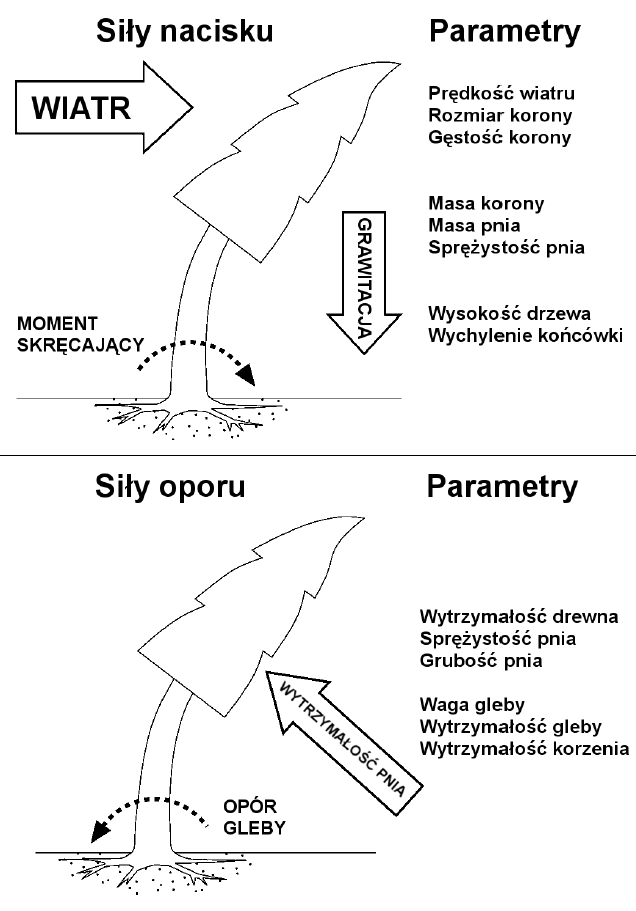
\includegraphics[scale=0.45]{HWIND1}
	\caption{Rozkład sił działających na drzewo dla modelu HWIND. Źródło:~\cite{chm_mgza}.}

\end{figure} 

Rysunek~\ref{fig:hwindScheme1} przedstawia siły działające na drzewo. Dokonany został podział na siły poziome i ~pionowe.
Pod naporem wiatru drzewo ugina się do momentu osiągnięcia punktu krytycznego, gdy siły nacisku (siła wiatru, siła grawitacji) zrównają się z ~siłami oporu (wytrzymałość pnia, wytrzymałość gleby wokół korzenia).

W celu wyznaczenia maksymalnego momentu skręcającego i ~granicznej prędkości wiatru przy której nastąpi zniszczenie drzewa, podzielone zostały one na 1~metrowe segmenty, dla których wyznaczone zostaną wartości sił.


\subsection{Siły nacisku}

Całkowita pozioma siła wiatru $F_w$ uzyskana zostaje poprzez sumowanie wartości siły wiatru obliczonej osobno dla każdego 1~metrowego segmentu~\cite{hpsk_hwind}. Siła dla poszczególnego segmentu uzyskiwana jest ze wzoru:
\begin{equation}
\label{eq:windForce}
 	F_w(z) = \frac{1}{2}C_d  \rho v_h^2 A(z)
\end{equation}
gdzie
\begin{description}
	\item[$C_d$] -- współczynnik tarcia
	\item[$\rho$ ]-- gęstość powietrza
	\item[$v_h$ ]-- prędkość pozioma dla danego segmentu
	\item[$A(z)$]-- przewidywana wielkość korony drzewa stawiająca opór wiatrowi
\end{description}

W celu uproszczenia obliczeń dokonana została aproksymacja powierzchni korony drzewa przez trójkąt równoramienny (świerk pospolity). Pole powierzchni pnia jest reprezentowane przez prostokąt. Model ten przedstawia rysunek~\ref{fig:hwindScheme2}.

\begin{figure}[!h]
\label{fig:hwindScheme2}
	\center
	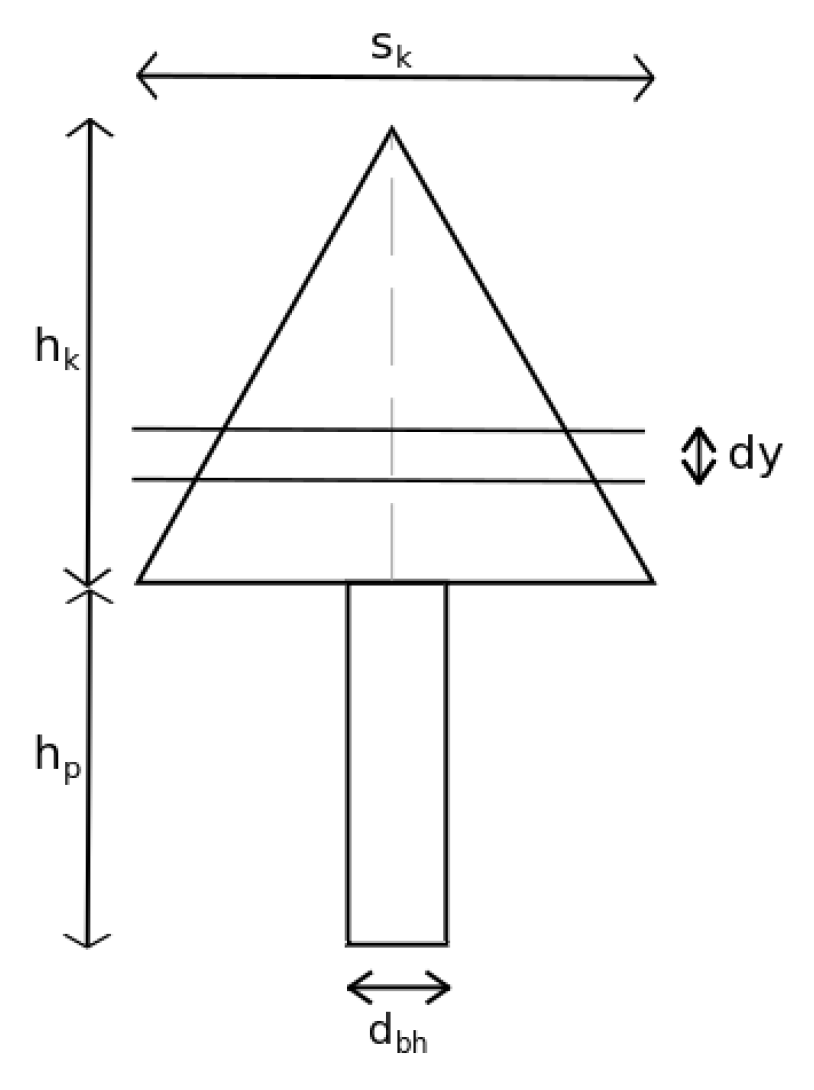
\includegraphics[scale=0.35]{HWIND2}
	\caption{Model powierzchni stawiającej opór wiatrowi. $s_k$ oznacza szerokość korony, $h_k$ -- wysokość korony, $h_p$ -- wysokość pnia, $d_{bh}$ -- średnicę pnia, $d_y$ -- wycinek powierzchni o wysokości $1m$ użyty przy w modelu HWIND. Źródło:~\cite{chm_mgza}.}

\end{figure} 

W modelu należy uwzględnić fakt, iż pod wpływem wiatru powierzchnia korony ulega zmniejszeniu~\cite{hpsk_hwind}. Redukcja powierzchni wynosi $20\%$ dla prędkości mniejszych od $11 \frac{m}{s}$, dla 
większych od $20\frac{m}{s}$ -- $60\%$. Dla wartości pomiędzy nimi współczynnik przepływu wiatru $S_t$ jest wyznaczany z następującego wzoru:
\begin{equation}
\label{eq:windFlow}
	 S_t(z) = 0.044444v(z) - 0.28889
\end{equation}
gdzie
\begin{description}
	\item[$v(z)$] -- prędkość wiatru na wysokości z
\end{description}

Powierzchnia $A(z)$ wyznaczana jest przez jej iloczyn ze współczynnikiem $S_t$.
\\

Siła grawitacji wyznaczana jest dla każdego segmentu drzewa, a następnie sumowana. Wyznaczana jest ze wzoru:
\begin{equation}
\label{eq:gravityForce}
	F_g(z) = m_c g
\end{equation}
gdzie
\begin{description}
	\item[$m_c$] -- masa korony drzewa
	\item[$g$] -- przyspieszenie ziemskie
\end{description}


\subsection{Maksymalny moment skręcający drzewa}

Maksymalny moment skręcający drzewa~$B_{max}(z)$ wyznaczamy dla każdego segmentu poprzez sumę siły wiatru~$F_w(z)$ pomnożonej przez wysokość~$\Delta z$, oraz siły grawitacji~$F_g(z)$ pomnożonej przez odchylenie czubka drzewa od pionu~$x(z)$~\cite{chm_ang}. Suma następnie zostaje pomnożona przez stosunek między maksymalnym, a średnim momentem ugięcia~$f_{gust}$ oraz stosunek pomiędzy maksymalnym, a średnim współczynnikiem odległości pomiędzy drzewami~$f_{gap}$. Zależność ta jest wyrażona następującym wzorem:

\begin{equation}
\label{eq:bendMoment}
	B_{max}(z) = f_{gust} f_{gap} [ F_w(z) \Delta z + F_g(z) x(z)]
\end{equation}

Odchylenie czubka od pionu używane w powyższym wzorze~(\ref{eq:bendMoment}) wyznaczane jest za pomocą wzoru~\cite{chm_ang}:
\begin{equation}
	\label{eq:crovnDeviation}
	 x(z) =
	\left\{
	\begin{array}{l r}
  		\frac{F_w a^2h(3- \frac{a}{h} - \frac{3l(z)}{h} }{6 \cdot MOE \cdot I} 	& \text{dla} \; z \leq a\\
	    	\frac{F_w a^3 (2-\frac{3(l(z)-b)}{a} + \frac{(l(z) - b)^3}{a^3}}{6 \cdot MOE \cdot I} & \text{dla} \; z > a\\
	  \end{array} \right.
\end{equation}
gdzie
\begin{description}
	\item[$a$] -- wysokość środka korony
	\item[$h$] -- wysokość drzewa
	\item[$l(z)$] -- odległość od czubka drzewa na wysokości $z$
	\item[$MOE$] -- współczynnik elastyczności drzewa
	\item[$I$] -- powierzchniowy moment bezwładoności ($I = \pi \frac{d_{bh}^4}{64}$, gdzie $d_{bh}$ to średnica drzewa na wysokości $1.3m$
	\item[$b$] -- odległość między czubkiem drzewa, a środkiem korony
\end{description}

Jak podaje źródło~\cite{hp_hwind} drzewa zachowują się inaczej pod napływem wiatru w zależności od tego jaka odległość dzieli je od ściany lasu. Proporcje zmian wyrażają wzory~(\ref{eq:gust}) oraz~(\ref{eq:gap}):

Dla momentu ugięcia:
\begin{equation}
\label{eq:gust}
 \begin{array}{c}
	Gust_{mean} = (0.68 \frac{s}{h} - 0.0385) + (-0.68\frac{s}{h} + 0.4875)(1.7239\frac{s}{h} + 0.0316)^{\frac{x}{h}} \\
	Gust_{max} = (2.7193\frac{s}{h} - 0.061) + (-1.273\frac{s}{h} + 9.9701)(1.1127\frac{s}{h} + 0.0311)^{\frac{x}{h}} \\
	f_{gust} = \frac{Gust_{max}}{Gust_{mean}}
  \end{array} 
\end{equation}
gdzie
\begin{description}
	\item[$s$] -- odległość między drzewami
	\item[$h$] -- średnia wysokość drzew w lesie
\end{description}

Dla współczynnika odległości pomiędzy drzewami:
\begin{equation}
\label{eq:gap}
\begin{array}{c}
	Gap_{mean} = \frac{0.001 + 0.001p^{0.562}}{0.00465} \\
	Gap_{max} = \frac{0.0072 + 0.0064 p^{0.3467}}{0.0214} \\
	f_{gap} = \frac{Gap_{max}}{Gap_{mean}}
\end{array} 
\end{equation}
gdzie
\begin{description}
	\item[$p$] -- szerokość pasa wolnej przestrzeni przed ścianą lasu.
\end{description}

\subsection{Siły oporu}

Wyznaczenie wartości sił oporu drzewa dokonane zostało na podstawie wzorów~(\ref{eq:trunkResistance}) oraz~(\ref{eq:rootResistance}).
Pień drzewa nie pęka do momentu w którym siła wiatru $F_w$ nie rozerwie włókien w zewnętrznych partiach kory. Wytrzymałość wyznacza
się na wysokości $1.3m$ (wysokość klatki piersiowej człowieka)~\cite{hpsk_hwind}, jest ona reprezentowana przez współczynnik pękania drewna $MOR$.

Wytrzymałość pnia:
\begin{equation}
\label{eq:trunkResistance}
	M_{bk} = \frac{\pi}{32} MOR d^3_{bh}
\end{equation}
gdzie
\begin{description}
	\item[$MOR$] -- współczynnik pękania drewna
	\item[$d_{bh}$] -- średnica drzewa na wysokości $1.3m$
\end{description}

Wytrzymałość korzenia wyznaczana jest w następujący sposób:
\begin{equation}
\label{eq:rootResistance}
	M_{ov} = \frac{g R_{mass} R_{depth}}{f_{RW}}
\end{equation}
gdzie
\begin{description}
	\item[$g$] -- przyspieszenie ziemskie
	\item[$R_{mass}$] -- masa korzenia
	\item[$R_{depth}$] -- głębokość korzenia
	\item[$f_{RW}$] -- stosunek wagi gleby do masy drzewa
\end{description}

Gdy moment ugięcia~(\ref{eq:bendMoment}) przekroczy wytrzymałość pnia~(\ref{eq:trunkResistance}) drzewo zostanie złamane. Gdy moment ugięcia przekroczy wytrzymałość gleby wokół korzeni~(\ref{eq:rootResistance}) -- drzewo zostanie wyrwane.

W projekcie symulacja dokonana została dla sosny zwyczajnej. Dla niej też zostały dobrane charakterystyczne wartości parametrów.


